\chapter{Open Problems and Research Directions}
\label{ch:open-problems}

\abstract*{Post-quantum cryptography is a field in rapid motion.  This final chapter surveys the principal open problems and research directions that will shape the discipline over the coming decades.  We examine quantum cryptanalysis of lattice problems, physical side-channel research on PQC implementations, hardware optimization for constrained devices, the engineering challenge of cryptographic agility, contingency planning for new mathematical breaks, and long-term visions for the quantum internet era.  The chapter concludes with a numbered catalogue of concrete open problems suitable for doctoral research.}

\abstract{Post-quantum cryptography is a field in rapid motion.  This final chapter surveys the principal open problems and research directions that will shape the discipline over the coming decades.  We examine quantum cryptanalysis of lattice problems, physical side-channel research on PQC implementations, hardware optimization for constrained devices, the engineering challenge of cryptographic agility, contingency planning for new mathematical breaks, and long-term visions for the quantum internet era.  The chapter concludes with a numbered catalogue of concrete open problems suitable for doctoral research.}

% =============================================================
% SOURCE: notes.tex §6.1, §6.3 (lines 7877–9409)
% REUSE: ~50%. Added concrete numbered open problems,
%        recent developments 2024-2025.
% =============================================================


\section{Quantum Cryptanalysis}
\label{sec:quantum-cryptanalysis}

Every cryptographic system lives under a sword: the possibility that someone will find a faster way to break it.  For RSA and elliptic-curve cryptography, that sword fell decades ago in theory---Shor's algorithm~\cite{Shor1997} factors integers and computes discrete logarithms in polynomial time on a quantum computer.  The only reprieve is engineering: no quantum machine yet has the scale to execute the attack.  Lattice-based cryptography was chosen as the successor precisely because no analogous quantum algorithm is known.  But ``not known'' is not ``impossible,'' and the question of whether quantum computers can efficiently solve lattice problems is arguably the most important open question in all of cryptography.

What makes this question so difficult is the nature of the gap.  Shor's algorithm succeeds because factoring and discrete logarithms are instances of the abelian hidden subgroup problem, and quantum Fourier transforms over abelian groups are efficient.  Lattice problems, by contrast, are related to \emph{non-abelian} hidden subgroup problems, where quantum Fourier transforms over the relevant groups are not known to help.  The challenge is not merely to find a faster algorithm, but to discover an entirely new structural insight---a way to make quantum interference reveal short lattice vectors the way it reveals hidden periods.

\subsection{The Quantum Algorithm Toolkit}
\label{subsec:quantum-toolkit}

Before asking what quantum computers might achieve against lattices, we should take stock of what quantum algorithms can do at all.  The known families relevant to cryptanalysis are surprisingly few\index{quantum algorithms!toolkit}:
\begin{enumerate}
\item \textbf{Hidden subgroup algorithms} (Shor): exponential speedup for abelian hidden subgroup problems.  Lattice problems are related to \emph{non-abelian} hidden subgroup problems, for which no efficient quantum algorithm is known~\cite{Regev2009}.
\item \textbf{Grover search}: a generic $\sqrt{N}$ speedup for unstructured search.  Applied to lattice sieving, Grover's algorithm reduces the exponent from $2^{0.292n}$ to approximately $2^{0.265n}$~\cite{Laarhoven2015}.
\item \textbf{Quantum walks}: polynomial speedups for graph-based search, applicable to certain enumeration subroutines.
\item \textbf{Quantum sampling}: algorithms such as HHL that solve linear systems exponentially fast under favourable conditions.
\end{enumerate}

The striking feature of this toolkit is its narrowness.  Decades of quantum algorithm research have produced, for cryptanalytic purposes, exactly one transformative technique (hidden subgroup methods) and several that offer modest polynomial speedups.  This is not for lack of trying---it reflects something deep about the structure of quantum computation.

\begin{svgraybox}
\textbf{The gap.}
There is a conspicuous absence in this list: no quantum algorithm exploits the algebraic structure of lattice problems in the way Shor exploits the group structure of $\Z_N^*$.  Closing---or proving the impossibility of closing---this gap is the central challenge of quantum cryptanalysis\index{quantum cryptanalysis}.
\end{svgraybox}

A breakthrough could come from an unexpected direction.  Perhaps the geometry of lattices admits a quantum encoding that we have not yet imagined.  Perhaps a new model of quantum computation---topological, measurement-based, or hybrid classical-quantum---will make visible a structure that the circuit model obscures.  Or perhaps lattice problems are genuinely hard for quantum computers, and the absence of progress reflects a real barrier rather than a failure of imagination.  Distinguishing between these possibilities is the work of the coming decades.

\subsection{Quantum Speedups for Sieving and Enumeration}
\label{subsec:quantum-sieving}

If no transformative quantum algorithm exists for lattice problems, the best we can hope for is to accelerate the known classical approaches.  Classical lattice sieving algorithms find short vectors by generating exponentially many lattice vectors and combining those that are close together.  The best classical sieving algorithms run in time $2^{0.292n + o(n)}$.  Applying Grover search to the nearest-neighbour subroutine yields a quantum sieving complexity of approximately $2^{0.265n + o(n)}$, at the cost of exponential quantum memory~\cite{Laarhoven2015}.

\begin{definition}[Quantum Sieving Complexity]
\label{def:quantum-sieving}
\index{sieving!quantum}
Let $T_{\mathrm{class}}(n) = 2^{c_1 n + o(n)}$ be the classical sieving time and $T_{\mathrm{quant}}(n) = 2^{c_2 n + o(n)}$ the quantum sieving time.  Current best known values are $c_1 \approx 0.292$ and $c_2 \approx 0.265$.  The \emph{quantum sieving advantage} is the ratio $c_1 / c_2 \approx 1.10$.
\end{definition}

A 10\% reduction in the exponent is significant but far from the exponential collapse that Shor inflicts on RSA.  To put it concretely: for the lattice dimensions relevant to ML-KEM-768, the quantum sieving advantage shaves roughly 20 bits off the security level---enough to matter for parameter selection, but not enough to threaten the scheme's viability.  For enumeration-based algorithms, quantum walks on the enumeration tree can provide a modest polynomial speedup, but the overall complexity remains $2^{\Theta(n)}$.

The deeper question is whether this 10\% is the end of the story or merely the beginning.  Could a cleverer use of quantum resources---better nearest-neighbour data structures, more efficient quantum memory access, or entirely new sieving strategies that are natively quantum---push the exponent significantly lower?  No concrete proposal has achieved this, but neither has anyone proved it impossible.

\subsection{Quantum Walks on Lattice Graphs}
\label{subsec:quantum-walks}

Quantum walk algorithms\index{quantum walks} offer an alternative approach that sidesteps the Grover framework entirely.  The idea is to define a graph whose vertices correspond to lattice vectors and whose edges connect ``close'' pairs, then deploy a quantum walk to search for short vectors.  The difficulty is fundamental: the graph has $2^{\Theta(n)}$ vertices, and quantum walks provide at best a quadratic speedup over classical random walks on generic graphs.

Recent work has explored whether \emph{structured} quantum walks---exploiting the periodicity of the lattice---can do better.  An analogy from condensed-matter physics is suggestive: Bloch's theorem shows that the periodicity of a crystal lattice constrains the electron wavefunctions to Bloch waves.  If a similar structural constraint could be imposed on a quantum walk over the lattice graph, it might yield a super-quadratic speedup.  No concrete algorithm of this type is known.

The analogy, however, is more tantalising than it may first appear.  In a physical crystal, periodicity creates band structure, and band structure creates forbidden and allowed energy regions that profoundly shape transport properties.  A lattice in the cryptographic sense has its own periodicity---the lattice vectors tile space---and a quantum walk that respects this periodicity might exhibit analogous transport phenomena.  Whether these phenomena can be harnessed for finding short vectors remains entirely open.  The tools exist in mathematical physics; what is missing is the bridge to algorithmic design.

\subsection{The SVP Holy Grail}
\label{subsec:svp-holy-grail}

All of the preceding discussion converges on a single question that looms over the entire field.

\begin{svgraybox}
\textbf{The SVP question.}
Is there a polynomial-time quantum algorithm for \svp{}\index{SVP!quantum complexity}?  A positive answer would break all lattice-based cryptography.  A negative answer---a proof that \svp{} is hard even for quantum computers---would place lattice-based cryptography on the firmest possible theoretical footing.  Neither result appears within reach.
\end{svgraybox}

Several intermediate results constrain what is possible.  The best known quantum lower bound for exact \svp{} is trivial ($\Omega(n)$, the cost of reading the input).  On the upper-bound side, there is no known quantum algorithm that beats $2^{0.265n}$ asymptotically.  Gidney and Eker\aa~\cite{GidneyEkera2021} have provided sharp quantum resource estimates for Shor's algorithm against RSA and elliptic curves, but comparable resource analyses for quantum lattice attacks remain incomplete---a significant gap in the literature.

We are, in a sense, building an entire cryptographic infrastructure on a conjecture: that lattice problems are hard for quantum computers.  The evidence for this conjecture is substantial---decades of effort by talented researchers have failed to refute it---but evidence is not proof.  The field proceeds, as it must, on the best available knowledge, while keeping one eye on the horizon for any sign that the conjecture might be wrong.


%% ================================================================
\section{Physical Side-Channel Research}
\label{sec:physical-research}

The previous sections asked whether the \emph{mathematics} of PQC can be broken.  This section asks a different and equally important question: can the \emph{physics} of PQC implementations be exploited?  Cryptographic implementations leak information through physical channels---power consumption, electromagnetic (EM) radiation, timing, and cache behaviour---and post-quantum algorithms introduce new side-channel surfaces that are not yet fully understood\index{side-channel analysis!PQC}.

The transition from RSA and elliptic curves to lattice-based schemes is not merely a change of mathematical assumptions; it is a change of computational workload.  Where classical schemes perform modular exponentiations over large integers, PQC schemes perform polynomial arithmetic over moderate-sized rings.  The leakage characteristics of these operations are fundamentally different, and the countermeasures developed over two decades for classical schemes do not transfer automatically.  Understanding this new leakage landscape is urgent: the algorithms are being standardised now, and implementations are being deployed into hardware that will be in the field for a decade or more.

\subsection{Electromagnetic Analysis of PQC}
\label{subsec:em-analysis}

The NTT butterfly operations at the heart of \mlwe{}-based schemes such as ML-KEM produce characteristic EM signatures.  Each butterfly involves a modular multiplication whose operand values influence switching activity on the data bus.  Near-field EM probes can resolve individual butterfly stages, potentially recovering polynomial coefficients that encode the secret key.

\begin{example}[EM Leakage in NTT]
\label{ex:em-ntt}
\index{NTT!side-channel leakage}
Consider an NTT of length $n = 256$ over $\Zq$ with $q = 3329$ (the ML-KEM parameter set).  The NTT consists of $\log_2 n = 8$ stages, each performing $n/2 = 128$ butterfly operations.  An EM probe positioned over the arithmetic unit of an unprotected microcontroller can distinguish twiddle-factor multiplications involving small coefficients (low Hamming weight) from those involving large coefficients, leaking partial information about the secret polynomial after as few as 1\,000 traces.
\end{example}

The implications extend beyond a single attack.  The NTT is not an optional component---it is the computational backbone of ML-KEM and ML-DSA, executed during every key generation, encapsulation, and signing operation.  Any EM vulnerability in the NTT is therefore a vulnerability in the entire scheme.  Protecting it requires understanding not just which coefficients leak, but how the leakage propagates through the NTT's butterfly structure and how it compounds across multiple operations with the same key.

\subsection{Deep Learning for Side-Channel Attacks}
\label{subsec:deep-learning-sca}

Classical side-channel attacks require the analyst to identify exploitable leakage points manually---a process that demands both domain expertise and considerable effort.  Deep learning\index{deep learning!side-channel attacks} models---convolutional and recurrent neural networks---upend this paradigm by learning leakage models directly from raw power or EM traces, bypassing the need for expert feature engineering.  For PQC implementations, this shift is particularly consequential because:
\begin{itemize}
\item The leakage model for polynomial arithmetic is more complex than for classical modular exponentiation.
\item Masking countermeasures that are effective against classical template attacks may be insufficient against neural-network-based profiling.
\item The large key and ciphertext sizes of PQC schemes produce longer traces with more potential leakage points.
\end{itemize}

The concern is not speculative.  Recent experiments have demonstrated that deep learning models can extract secret keys from masked PQC implementations using fewer traces than classical statistical attacks.  The arms race between attack and defence in this domain is accelerating, and the defensive side is not clearly winning.

\subsection{Physics-Informed Countermeasures}
\label{subsec:physics-countermeasures}

Effective countermeasures require understanding the physical leakage mechanism, not merely the algorithmic one.  A masking scheme that is provably secure in an idealised leakage model may fail spectacularly when the leakage model does not match the actual physics of the chip.  Examples of physics-informed approaches include:
\begin{enumerate}
\item \textbf{Dual-rail logic}\index{dual-rail logic}: balancing switching activity at the transistor level so that every operation dissipates the same energy regardless of operand values.
\item \textbf{EM shielding}: designing package-level Faraday cages calibrated to the frequencies at which NTT operations emit.
\item \textbf{Noise injection}: adding controlled random switching activity whose spectrum masks the signal of interest.  The noise budget must be set by modelling the channel capacity of the EM side channel.
\end{enumerate}

Each of these approaches carries costs---in area, in power, in design complexity---and none is a silver bullet.  The research challenge is to find the right combination for each deployment context, from billion-unit smart cards where every gate counts to server-class hardware where area is cheap but throughput is paramount.

\subsection{Quantum Side Channels}
\label{subsec:quantum-side-channels}

As quantum computers begin to execute cryptographic algorithms, they introduce an entirely new class of side channels\index{side-channel analysis!quantum} that has no precedent in classical hardware:
\begin{itemize}
\item \textbf{Qubit crosstalk:} in superconducting processors, the resonant frequency of a qubit shifts depending on the state of its neighbours, potentially leaking information about the computation.
\item \textbf{Photon statistics in QKD:} detector timing jitter and after-pulsing probabilities depend on photon energy, creating a side channel in quantum key distribution systems.
\item \textbf{Cryogenic thermal signatures:} heat dissipation in dilution refrigerators varies with the number and type of gate operations, providing a coarse-grained side channel on quantum algorithm execution.
\end{itemize}

These quantum side channels are largely unexplored from a cryptanalytic perspective.  The physics community understands the mechanisms intimately---crosstalk is a major engineering challenge in scaling quantum processors---but has not yet examined them through the lens of an adversary.  This intersection of quantum hardware engineering and cryptographic security represents one of the most fertile and least explored research frontiers in the field.


%% ================================================================
\section{Hardware Optimization}
\label{sec:hardware}

Moving from theory to practice, we confront a blunt engineering reality: PQC algorithms are more computationally expensive than their classical predecessors, and the devices that must run them are not getting bigger.  Deploying PQC on resource-constrained devices---smart cards, IoT sensors, embedded controllers---requires hardware implementations that meet strict area, power, and latency budgets\index{hardware!PQC optimization}.  The question is not whether PQC can be implemented in hardware; it is whether it can be implemented within the budgets that the application demands.

\subsection{FPGA and ASIC Implementations of NTT}
\label{subsec:ntt-hardware}

The Number Theoretic Transform\index{NTT!hardware} dominates the computational cost of \mlwe{}-based schemes, just as modular exponentiation dominated the cost of RSA.  On a general-purpose CPU, an NTT of length $n = 256$ with $q = 3329$ requires approximately $n \log_2 n = 2048$ butterfly operations, each involving a modular multiplication and addition.  A dedicated hardware butterfly unit can execute one butterfly per clock cycle, completing the full NTT in $\log_2 n = 8$ cycles when $n/2 = 128$ butterfly units operate in parallel.

\begin{table}[t]
\caption{NTT implementation tradeoffs for ML-KEM ($n=256$, $q=3329$)}
\label{tab:ntt-hw}
\begin{tabular}{p{3cm}p{2.5cm}p{2.5cm}p{2.5cm}}
\hline\noalign{\smallskip}
\textbf{Architecture} & \textbf{Area (kGE)} & \textbf{Latency ($\mu$s)} & \textbf{Energy (nJ)} \\
\noalign{\smallskip}\svhline\noalign{\smallskip}
Software (ARM Cortex-M4) & --- & $\sim$100 & $\sim$10\,000 \\
1 butterfly unit & $\sim$5 & $\sim$10 & $\sim$50 \\
4 butterfly units & $\sim$15 & $\sim$3 & $\sim$20 \\
128 butterfly units & $\sim$400 & $\sim$0.1 & $\sim$10 \\
\noalign{\smallskip}\hline
\end{tabular}
\end{table}

The numbers in Table~\ref{tab:ntt-hw} reveal a classic area--latency tradeoff, but they also tell a more nuanced story.  Energy decreases with parallelism even as area grows, because the parallel design completes faster and spends less time in energy-consuming idle states.  For IoT applications where energy is the binding constraint, the single-butterfly design is often preferred; for high-throughput servers, fully parallel implementations are justified.  The design space between these extremes is large and largely unexplored---finding Pareto-optimal points for specific deployment scenarios is an active research area.

\subsection{Gaussian Sampling Hardware}
\label{subsec:gaussian-hw}

Schemes based on Gaussian noise (including earlier NTRU variants and certain signature schemes) require sampling from a discrete Gaussian distribution\index{Gaussian sampling!hardware}.  This is a deceptively difficult problem in hardware.  The sampler must simultaneously satisfy three competing requirements:
\begin{itemize}
\item \textbf{Statistical quality:} the output distribution must be indistinguishable from ideal to prevent statistical side-channel attacks.
\item \textbf{Constant-time execution:} rejection sampling introduces data-dependent timing; hardware implementations must mask this variation.
\item \textbf{Entropy consumption:} each sample requires fresh random bits; the TRNG must keep pace with the sampling rate.
\end{itemize}

Cumulative Distribution Table (CDT) sampling and the Knuth--Yao algorithm are the two dominant hardware approaches.  CDT sampling uses a precomputed table and a single comparison per sample, achieving constant time at the cost of table storage.  The Knuth--Yao algorithm is more memory-efficient but requires a variable number of random bits per sample.  Neither approach is clearly superior---the choice depends on the available silicon budget and the paranoia level of the threat model.

\subsection{Energy-Efficient PQC for IoT}
\label{subsec:iot-energy}

For battery-powered IoT devices, the energy cost of a single key encapsulation may determine whether PQC is feasible at all\index{IoT!PQC energy}.  ML-KEM-512, the lightest NIST-standardised parameter set, requires approximately 150\,000 arithmetic operations for encapsulation.  On an ARM Cortex-M0+ at 1.8\,V and 16\,MHz, this translates to roughly 10\,$\mu$J---orders of magnitude more than an ECDH key exchange.

This gap is not merely inconvenient; it is potentially disqualifying.  A sensor node running on a coin-cell battery that performs one key exchange per hour can afford 10\,$\mu$J.  A node that performs one per second cannot.  Reducing this energy cost through algorithmic, architectural, and circuit-level optimisation is an active research area with direct practical impact---one that will determine whether billions of deployed IoT devices can participate in a post-quantum world or must be left behind.


%% ================================================================
\section{Cryptographic Agility}
\label{sec:crypto-agility}

History teaches that every cryptographic algorithm eventually falls\index{cryptographic agility}.  DES lasted 20 years.  MD5 lasted 13.  SHA-1 lasted 12 from the first theoretical cracks to practical collision.  The ability to replace algorithms quickly and safely---\emph{cryptographic agility}---is therefore not a luxury but a survival requirement.  Yet most deployed systems treat their cryptographic algorithms as load-bearing walls rather than replaceable components, and the resulting brittleness has turned every past algorithm deprecation into a multi-year ordeal.

Figure~\ref{fig:ch17-algorithm-decay} plots the lifespans of several major cryptographic algorithms, illustrating the recurring pattern: every algorithm is eventually weakened or broken, and the trend line shows no sign of stopping.

\begin{figure}[t]
\centering
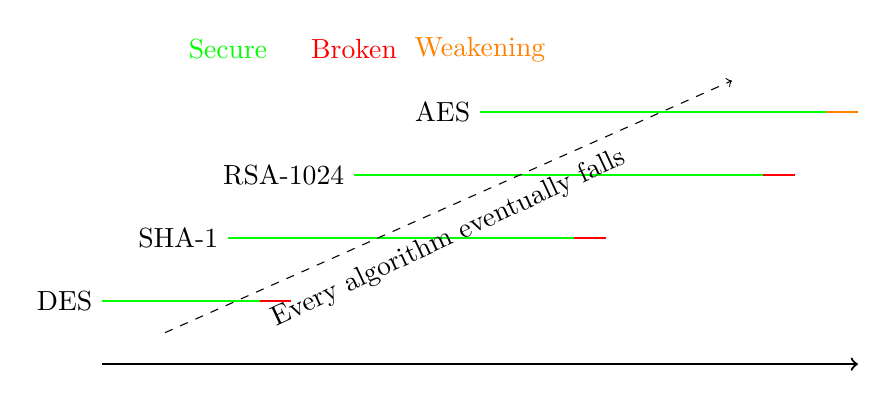
\begin{tikzpicture}[scale=0.8]
    % Timeline
    \draw[thick, ->] (0,0) -- (12,0);

    % Algorithm lifetimes
    \draw[thick, green] (0,1) -- (3,1);
    \node[left] at (0,1) {DES};
    \draw[thick, red] (2.5,1) -- (3,1);

    \draw[thick, green] (2,2) -- (8,2);
    \node[left] at (2,2) {SHA-1};
    \draw[thick, red] (7.5,2) -- (8,2);

    \draw[thick, green] (4,3) -- (11,3);
    \node[left] at (4,3) {RSA-1024};
    \draw[thick, red] (10.5,3) -- (11,3);

    \draw[thick, green] (6,4) -- (12,4);
    \node[left] at (6,4) {AES};
    \draw[thick, orange] (11.5,4) -- (12,4);

    % Legend
    \node[green] at (2,5) {Secure};
    \node[red] at (4,5) {Broken};
    \node[orange] at (6,5) {Weakening};

    % Pattern
    \draw[dashed, ->] (1,0.5) -- (10,4.5);
    \node[rotate=25] at (5.5,2) {Every algorithm eventually falls};
\end{tikzpicture}
\caption{The inevitable decay of cryptographic algorithms.  Each algorithm enjoys a period of trusted security (green) before cryptanalytic advances weaken (orange) or break (red) it.  No algorithm has proven permanent; cryptographic agility is the only sustainable defence.}
\label{fig:ch17-algorithm-decay}
\end{figure}

\subsection{Algorithm-Agnostic Design}
\label{subsec:agnostic-design}

What would it mean for a system to be truly algorithm-agnostic?  Not merely to support multiple algorithms, but to treat the choice of algorithm as a runtime configuration parameter rather than a compile-time decision.

\begin{definition}[Cryptographic Agility]
\label{def:crypto-agility}
A system exhibits \emph{cryptographic agility}\index{cryptographic agility!definition} if:
\begin{enumerate}
\item Algorithms are identified by negotiable object identifiers (OIDs), not hard-coded implementations.
\item Multiple algorithms can coexist in the same deployment.
\item Algorithm transitions require configuration changes, not code changes.
\item Monitoring infrastructure tracks which algorithms are in active use.
\end{enumerate}
\end{definition}

Achieving agility requires abstracting the cryptographic layer behind a stable interface.  The provider pattern---where algorithm implementations are loaded dynamically based on policy---is the standard architectural approach.  However, agility introduces its own risks: a larger algorithm menu expands the attack surface (downgrade attacks) and increases testing burden.  The engineering challenge is to gain the flexibility of agility without the fragility that comes from supporting too many options.

\subsection{Protocol Negotiation}
\label{subsec:protocol-negotiation}

TLS~1.3\index{TLS!agility} demonstrates effective protocol-level agility: the client advertises supported groups and signature algorithms, and the server selects the strongest mutually supported option.  Extending this mechanism to include PQC algorithms---as done in hybrid key exchange drafts---is straightforward in principle.  The challenges are operational:
\begin{itemize}
\item Larger key shares increase the ClientHello size, sometimes exceeding a single TCP segment and triggering fragmentation.
\item Certificate chains containing PQC signatures are significantly larger, straining bandwidth-limited links.
\item Negotiation must handle the case where a previously trusted algorithm is abruptly deprecated.
\end{itemize}

These are not theoretical concerns.  Early deployments of hybrid TLS have already encountered middleboxes that drop oversized ClientHellos, certificate verification failures due to unexpected signature algorithms, and interoperability problems between implementations at different stages of standards compliance.  The path from ``the protocol supports it'' to ``the internet works with it'' is long and paved with operational surprises.

\subsection{Lessons from SHA-1 and MD5}
\label{subsec:sha1-lessons}

The deprecation of MD5\index{MD5!deprecation} and SHA-1\index{SHA-1!deprecation} provides instructive---and sobering---precedents.  MD5 collision attacks were first demonstrated in 2004, yet MD5-signed certificates persisted in the Web PKI until at least 2012.  SHA-1 collisions were demonstrated in 2017 (the SHAttered attack); major browsers did not fully remove SHA-1 certificate support until 2019---two years after the break and twelve years after the first theoretical weaknesses.

\begin{svgraybox}
\textbf{Lesson.}
The time between a cryptographic break and the completion of migration is measured in years to decades, not days.  Systems that lack agility transform an algorithmic weakness into a systemic crisis.  The PQC transition is our opportunity to build agility into infrastructure \emph{before} it is needed.
\end{svgraybox}

The PQC transition differs from the SHA-1 and MD5 episodes in one crucial respect: we are migrating \emph{before} the break, not after.  This is unprecedented in the history of cryptography, and it gives us a window---narrow but real---to design the migration infrastructure correctly.  Whether we use that window well will determine whether the next cryptographic break is a managed transition or a global emergency.


%% ================================================================
\section{Preparing for New Breaks}
\label{sec:preparing-breaks}

The preceding section argued that agility is essential.  This section asks a harder question: what specifically should we be agile \emph{toward}?  The NIST PQC standards are based primarily on the hardness of lattice problems (\mlwe{}, \rlwe{}, Module-NTRU).  This is a deliberate bet---lattice problems have the strongest theoretical foundations and the best performance characteristics.  But it is a bet nonetheless, and responsible engineering demands a contingency plan.  What happens if these foundations crack?

\subsection{What if Module-LWE Breaks?}
\label{subsec:mlwe-break}

A polynomial-time algorithm for \mlwe{}\index{Module-LWE!break scenario} would invalidate ML-KEM and ML-DSA simultaneously, disabling both key encapsulation and digital signatures.  The impact would be comparable to a polynomial-time factoring algorithm in the pre-quantum era---but broader, because NIST has concentrated its standards on a single hardness assumption.  In the classical world, at least, RSA and Diffie--Hellman rested on different (though related) problems.  The lattice monoculture is efficient but fragile.

Fallback options under active standardisation or study include:
\begin{itemize}
\item \textbf{Code-based cryptography:} Classic McEliece (NIST round~4) rests on the hardness of decoding random linear codes, studied for over 45 years.  Key sizes are large (hundreds of kilobytes) but ciphertext sizes are competitive.
\item \textbf{Hash-based signatures:} SPHINCS$^+$ (standardised as SLH-DSA) requires only the security of a hash function---a minimal assumption.  Signature sizes are large ($\sim$8--50\,KB) but the scheme is a robust fallback.
\item \textbf{Multivariate-quadratic schemes:} These have a chequered history of breaks, but research continues on hardened variants.
\end{itemize}

None of these alternatives matches the performance of lattice-based schemes.  Classic McEliece keys are too large for many applications; SLH-DSA signatures are too slow for high-throughput signing.  The research imperative is clear: we need either to improve the efficiency of these fallback schemes or to identify new hardness assumptions that yield practical constructions.

\subsection{Defence in Depth}
\label{subsec:defence-depth}

The vulnerability of any single assumption motivates combining multiple assumptions so that an adversary must break all of them to compromise the system.

\begin{definition}[Cryptographic Defence in Depth]
\label{def:defence-depth}
\index{defence in depth}
A system employs \emph{cryptographic defence in depth} if it combines multiple independent hardness assumptions such that an adversary must break \emph{all} of them to compromise the system.  The standard realisation is \emph{hybrid} key exchange: the shared secret is the hash of a classical ECDH key and a PQC KEM key, so the system is secure as long as \emph{either} assumption holds.
\end{definition}

Hybrid modes are now supported in TLS (e.g., X25519+ML-KEM-768) and are recommended by multiple national agencies during the transition period.  The cost is modest: approximately double the computation and bandwidth of a single key exchange.  This is a price worth paying for insurance against a catastrophic break---but it is not free, and systems that adopt hybrid modes must budget for the overhead in their capacity planning.

\subsection{Monitoring Cryptanalysis}
\label{subsec:monitoring}

Defence in depth is a structural safeguard.  Monitoring is the operational one.  Early warning of approaching breaks requires systematic tracking of progress on several fronts\index{cryptanalysis!monitoring}:
\begin{enumerate}
\item \textbf{Lattice dimension records:} track the largest dimension in which \svp{} or \cvp{} has been solved exactly, and the approximation factors achieved in challenge lattices.
\item \textbf{Algorithmic improvements:} a reduction in the sieving exponent $c$ (currently $c \approx 0.292$ classically, $c \approx 0.265$ quantumly) would directly affect security estimates.
\item \textbf{Quantum hardware milestones:} logical qubit counts, error rates, and demonstrated algorithm execution times.
\item \textbf{New mathematical connections:} unexpected reductions between problems---such as a reduction from \mlwe{} to a problem known to be easy---would be a red flag.
\end{enumerate}

No single indicator will flash red the day before a break.  Cryptographic collapses are usually the culmination of a series of incremental advances, each individually unthreatening.  The discipline required is to track these increments systematically and to have the institutional courage to act when the trendline points toward danger---even when no individual result is yet alarming.


%% ================================================================
\section{The 50-Year Horizon}
\label{sec:horizon}

Cryptographic infrastructure protects data whose sensitivity may span decades: medical records, state secrets, financial archives, intellectual property.  A birth certificate issued today may need to be verifiable in 2076.  A classified intelligence assessment filed this year must remain confidential for at least 25 years, often 50.  Planning on this timescale forces us to reason about technologies and mathematical discoveries that do not yet exist\index{50-year horizon}, and to design systems that will survive surprises we cannot anticipate.

This is, in some ways, an absurd task.  Fifty years ago, public-key cryptography itself did not exist---Diffie and Hellman's seminal paper was still a year away.  The notion that we can predict the cryptographic landscape of 2076 is hubris.  Yet the alternative---building infrastructure that assumes today's assumptions will hold forever---is worse than hubris; it is negligence.  The goal is not to predict the future but to build systems that are robust to a wide range of futures.

Figure~\ref{fig:ch17-quantum-futures} sketches three plausible trajectories for quantum computing power over the coming decades.  Each scenario demands a different cryptographic strategy: exponential growth requires immediate and aggressive migration, linear growth allows a measured transition, and a plateau scenario relaxes urgency but does not eliminate it---because even modest quantum capability breaks some classical schemes.

\begin{figure}[t]
\centering
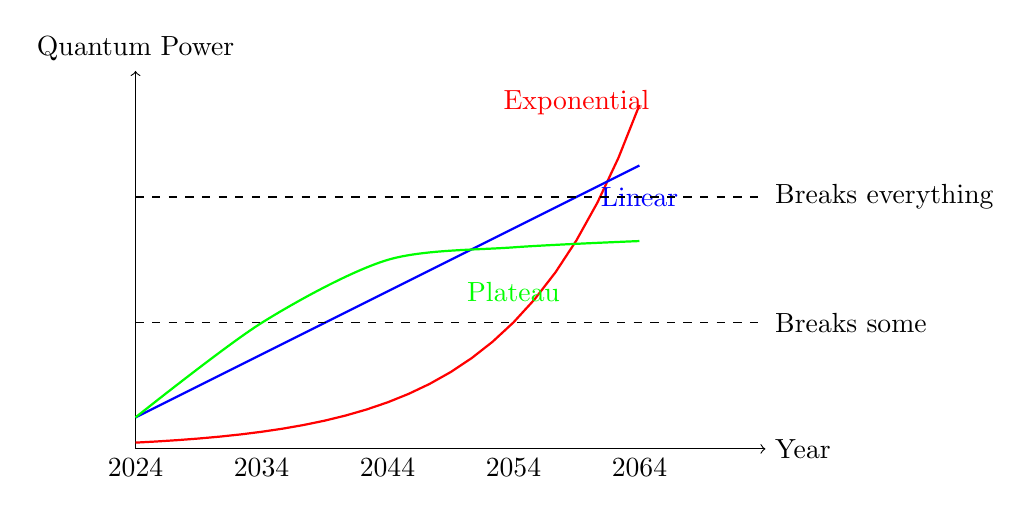
\begin{tikzpicture}[scale=0.8]
    % Axes
    \draw[->] (0,0) -- (10,0) node[right] {Year};
    \draw[->] (0,0) -- (0,6) node[above] {Quantum Power};

    % Scenarios
    % Exponential
    \draw[thick, red] plot[domain=0:8] (\x, {0.1*exp(0.5*\x)});
    \node[red] at (7,5.5) {Exponential};

    % Linear
    \draw[thick, blue] (0,0.5) -- (8,4.5);
    \node[blue] at (8,4) {Linear};

    % Plateau
    \draw[thick, green] plot[smooth] coordinates {
        (0,0.5) (2,2) (4,3) (6,3.2) (8,3.3)
    };
    \node[green] at (6,2.5) {Plateau};

    % Annotations
    \draw[dashed] (0,4) -- (10,4);
    \node[right] at (10,4) {Breaks everything};

    \draw[dashed] (0,2) -- (10,2);
    \node[right] at (10,2) {Breaks some};

    % Labels
    \foreach \x/\year in {0/2024, 2/2034, 4/2044, 6/2054, 8/2064} {
        \node[below] at (\x,0) {\year};
    }
\end{tikzpicture}
\caption{Three quantum futures, each requiring a different cryptographic strategy.  Exponential growth (red) demands immediate migration; linear growth (blue) allows a measured pace; a plateau (green) relaxes urgency but does not eliminate it, since even modest quantum capability breaks some classical schemes.}
\label{fig:ch17-quantum-futures}
\end{figure}

\subsection{The Quantum Internet}
\label{subsec:quantum-internet}

The most transformative development on the horizon is the quantum internet: a global network connecting quantum processors via entanglement distribution\index{quantum internet}.  A mature quantum internet would enable quantum key distribution (QKD) over arbitrary distances, offering information-theoretic key exchange---security guaranteed by the laws of physics rather than the conjectured hardness of a mathematical problem.

The appeal is obvious.  Information-theoretic security does not degrade with advances in computing or mathematics.  A key exchanged via QKD today will be just as secure against a quantum computer in 2076 as it is against a classical computer today.  For data that truly must remain secret for decades, this guarantee is qualitatively different from anything computational cryptography can offer.

However, QKD alone does not replace public-key cryptography.  It requires an authenticated classical channel (which itself needs PQC signatures), does not provide digital signatures, and its throughput is orders of magnitude below that of computational schemes.  A QKD link might exchange a few thousand key bits per second over a metropolitan fibre; a PQC key encapsulation runs in microseconds and requires no dedicated quantum hardware.  The realistic future is not one in which QKD replaces PQC, but one in which they coexist in a \emph{layered} security stack---PQC providing the bulk computational cryptography, QKD hardening the highest-sensitivity links where the cost and complexity are justified.

\subsection{Post-Quantum Plus Quantum: The Full Stack}
\label{subsec:full-stack}

The long-term security architecture, then, will not be a single technology but an integrated stack of complementary layers\index{security!full stack}:
\begin{enumerate}
\item \textbf{Physical layer:} QKD and quantum random number generation provide information-theoretic primitives.
\item \textbf{Computational layer:} PQC algorithms handle authentication, general-purpose encryption, and signatures.
\item \textbf{Protocol layer:} agile protocols negotiate the best available combination of physical and computational security.
\item \textbf{Policy layer:} automated monitoring and migration tools manage algorithm lifecycles.
\end{enumerate}

No single layer is sufficient.  QKD cannot authenticate; PQC relies on computational assumptions that may eventually fail; protocols without agility become liabilities; policy without automation is too slow.  Defence in depth across layers is the only sustainable strategy~\cite{Peikert2016}.

The analogy to network architecture is deliberate.  The TCP/IP stack succeeded not because any single layer was perfect, but because each layer could evolve independently while maintaining stable interfaces with its neighbours.  The cryptographic stack of the future must achieve the same modularity.  A breakthrough in quantum repeater technology should strengthen the physical layer without requiring changes to the PQC algorithms above it.  A new post-quantum signature scheme should slot into the computational layer without disrupting the QKD infrastructure below.  Achieving this clean separation of concerns---while maintaining the tight integration needed for security---is perhaps the grandest engineering challenge of the PQC era.

\subsection{Information-Theoretic vs.\ Computational Security}
\label{subsec:it-vs-comp}

Underlying these architectural questions is a philosophical one that has divided cryptographers since Shannon: should we aim for information-theoretic security (where no amount of computation can break the system) or accept computational security (where breaking the system requires more computation than an adversary can muster)?

\begin{table}[t]
\caption{Information-theoretic vs.\ computational security for long-term planning}
\label{tab:it-vs-comp}
\begin{tabular}{p{3cm}p{4.5cm}p{4.5cm}}
\hline\noalign{\smallskip}
\textbf{Criterion} & \textbf{Information-theoretic} & \textbf{Computational} \\
\noalign{\smallskip}\svhline\noalign{\smallskip}
Key management & Requires pre-shared or QKD keys & Public-key infrastructure \\
Bandwidth cost & One-time pad: $|K| \geq |M|$ & Compact ciphertexts \\
Assumption & None (physics only) & Hardness of a math problem \\
Scalability & Poor (point-to-point) & Excellent (public-key) \\
Longevity & Permanent & Until assumption fails \\
\noalign{\smallskip}\hline
\end{tabular}
\end{table}

The practical answer, as Table~\ref{tab:it-vs-comp} makes clear, is hybrid: information-theoretic security for the most sensitive, low-volume channels; computational security for the vast majority of communications.  The trade-off is not between good and bad, but between two kinds of risk.  Information-theoretic security eliminates computational risk but introduces physical risk (the security of QKD depends on correct modelling of the quantum channel and the absence of implementation flaws in the quantum hardware).  Computational security eliminates physical risk but introduces mathematical risk (the hardness assumption might fall).

The PQC transition is about securing the computational layer against quantum adversaries, while the parallel development of quantum networks strengthens the physical layer.  Fifty years from now, both layers will look very different from what we build today.  The measure of our success will not be whether we chose the right algorithms---we almost certainly will not have---but whether we built the right abstractions to let them be replaced gracefully when better ones arrive.


%% ================================================================
\section{Concrete Open Problems}
\label{sec:open-problem-list}

The following problems are open as of early 2026\index{open problems}.  Each combines a precise statement with a brief discussion of why the problem matters, what approaches have been tried, and where a new perspective might succeed.

\begin{enumerate}

\item \textbf{Quantum complexity of SVP.}
Determine the quantum query complexity of exact \svp{} in $n$ dimensions.  Is $2^{\Theta(n)}$ optimal, or does a sub-exponential quantum algorithm exist?  The best known quantum upper bound is $2^{0.265n + o(n)}$ from quantum sieving; no super-linear lower bound is known.  Even proving a $2^{\omega(\sqrt{n})}$ quantum lower bound would be a major advance~\cite{Regev2009}.

This is the foundational question of the field.  A sub-exponential quantum algorithm would require re-parameterising every lattice-based standard; a strong lower bound would justify the entire PQC programme on firm theoretical ground.  Either result would reshape the landscape.

\item \textbf{Tight reductions for Module-LWE.}
The security proof of ML-KEM reduces \mlwe{} to worst-case lattice problems, but the reduction incurs a polynomial loss in the security parameter~\cite{Peikert2016}.  Can this loss be eliminated?  Tight reductions would allow smaller parameters and thus more efficient schemes, directly impacting every deployment.

The polynomial loss is not merely an aesthetic blemish---it forces parameter choices to be conservative, adding kilobytes to keys and microseconds to operations across billions of devices.  Closing this gap would have immediate, tangible engineering consequences.

\item \textbf{Quantum resource estimates for lattice attacks.}
Provide end-to-end quantum resource estimates---logical qubits, T-gate count, circuit depth, wall-clock time under realistic error correction---for the best known quantum attacks on ML-KEM-768 and ML-KEM-1024.  Gidney and Eker\aa~\cite{GidneyEkera2021} performed this analysis for RSA-2048 and elliptic curves; the lattice case is missing.

Without these estimates, we are setting security parameters based on asymptotic analysis rather than concrete costs.  The RSA estimates revealed that Shor's algorithm requires fewer resources than previously assumed; a similar analysis for lattices could either confirm or challenge current parameter choices.

\item \textbf{Side-channel security of NTT implementations.}
Characterise the information-theoretic leakage of masked NTT implementations.  Specifically: for an NTT masked at order $d$, what is the minimum number of EM traces required to recover a secret coefficient, as a function of $d$ and the signal-to-noise ratio?  Current bounds are empirical, not theoretical.

Theoretical leakage bounds would transform side-channel protection from an empirical art into an engineering discipline, allowing designers to choose masking orders with provable security guarantees rather than relying on attack-and-patch cycles.

\item \textbf{Constant-time Gaussian sampling with minimal entropy.}
Design a constant-time discrete Gaussian sampler that is provably secure against timing side channels and consumes fewer than $2\lceil\log_2(\sigma)\rceil + 3$ random bits per sample, where $\sigma$ is the standard deviation.  The current best constructions consume significantly more.

Entropy is a scarce resource in constrained hardware.  A sampler that uses fewer random bits per sample directly reduces the load on the true random number generator, which is often the throughput bottleneck in embedded PQC implementations.

\item \textbf{Sub-linear-area NTT for constrained devices.}
Design an NTT hardware architecture for ML-KEM that fits within 3\,kGE (gate equivalents) while completing a full NTT in fewer than 5\,000 clock cycles.  Achieving this would make PQC viable on the smallest smart-card ICs.

Smart cards and similar constrained devices are deployed in the billions, and many must support cryptographic operations for a decade or more.  If PQC cannot fit on these devices, the post-quantum transition will leave a vast installed base unprotected.

\item \textbf{Formal verification of PQC implementations.}
Develop a formally verified (machine-checked) implementation of ML-KEM in a language suitable for embedded deployment (e.g., C or Rust).  The implementation must be verified for both functional correctness (agreement with the specification) and constant-time execution (absence of secret-dependent branching and memory access).

The history of cryptographic implementation is littered with bugs that formal methods could have caught---Heartbleed, Lucky~13, countless timing side channels.  A verified reference implementation would not only prevent such bugs but would serve as a trusted baseline against which other implementations can be validated.

\item \textbf{Hybrid protocol overhead bounds.}
Determine the minimum additional latency and bandwidth overhead of hybrid PQC/classical key exchange in TLS~1.3 as a function of network round-trip time and MTU.  Current empirical measurements vary widely; a clean analytical model validated against measurement would be valuable.

Hybrid key exchange is the recommended deployment mode during the transition, but the overhead is poorly characterised.  Network operators need reliable models to plan capacity, and protocol designers need them to optimise handshake flows.

\item \textbf{Worst-case to average-case reductions for code-based problems.}
The Ajtai-style worst-case to average-case connection that gives lattice-based cryptography its strong theoretical foundation~\cite{MicciancioGoldwasser2002} has no known analogue for code-based problems (syndrome decoding of random linear codes).  Establishing such a connection---or proving it impossible---would clarify the comparative theoretical footing of the two families.

Code-based cryptography is the leading fallback if lattice assumptions fail.  Without a worst-case to average-case reduction, its security rests on decades of failed attacks rather than on a provable connection to a well-studied hard problem.  Resolving this question would either elevate code-based cryptography to the same theoretical standing as lattice-based schemes or clarify why such standing is unattainable.

\item \textbf{Post-quantum oblivious transfer.}
Construct an efficient post-quantum oblivious transfer (OT) protocol with communication complexity sub-linear in the security parameter.  OT is a foundational primitive for secure multi-party computation; current PQC-based OT constructions are significantly less efficient than their classical counterparts.

Secure multi-party computation is increasingly used in privacy-preserving machine learning, auctions, and financial computations.  If OT remains expensive in the post-quantum setting, these applications will face a performance cliff when classical assumptions are deprecated.

\item \textbf{Quantum side-channel taxonomy.}
Develop a systematic taxonomy of side channels in superconducting and photonic quantum processors, including qubit crosstalk, readout crosstalk, and thermal signatures.  For each channel, determine the information leakage rate (bits per operation) and propose countermeasures.  No comprehensive framework exists.

As quantum computers begin executing cryptographic algorithms---both for attack (running Shor's algorithm) and defence (QKD, quantum random number generation)---the security of these computations against physical observers becomes a practical concern.  A taxonomy is the first step toward principled protection.

\item \textbf{Automated cryptographic migration.}
Design and evaluate a system that can automatically detect the use of deprecated cryptographic algorithms in a large code base ($> 10^6$ lines), propose replacements compatible with the existing API contracts, and verify that the replacement preserves functional behaviour.  Current migration efforts are overwhelmingly manual.

The SHA-1 deprecation took over a decade in part because every migration was a bespoke engineering effort.  Automated migration tooling would compress the timeline from years to weeks, transforming cryptographic agility from an aspiration to an operational reality.

\end{enumerate}


%% ================================================================
%% Exercises
%% ================================================================

\begin{prob}
\label{prob:ch15-quantum-resource}
Gidney and Eker\aa~\cite{GidneyEkera2021} estimate that factoring a 2048-bit RSA modulus requires approximately 20 million noisy qubits over 8 hours.  Suppose a quantum sieving algorithm for \svp{} in dimension $n$ requires $2^{0.265n}$ quantum operations, each implemented as a circuit of depth $D = \poly(n)$.  Under the surface-code error correction model with a physical error rate of $10^{-3}$, estimate the number of physical qubits and wall-clock time required to attack ML-KEM-768 (which targets 192-bit security, corresponding to $n \approx 700$ in the lattice dimension).  Compare with the Gidney--Eker\aa{} RSA estimate and discuss which system is more vulnerable in the medium term.
\end{prob}

\begin{prob}
\label{prob:ch15-agility}
Design a cryptographic agility framework for a web service currently using TLS~1.3 with X25519 and Ed25519.  Your framework must allow swapping to any NIST-standardised PQC algorithm within 48~hours of a break announcement.  Identify the components that need abstraction (TLS library, certificate infrastructure, key storage, monitoring) and the operational procedures required (key rotation, certificate reissuance, client compatibility testing).  Discuss the tradeoff between agility and the risk of downgrade attacks.
\end{prob}

\begin{prob}
\label{prob:ch15-hybrid-overhead}
Consider a TLS~1.3 handshake using hybrid key exchange (X25519 + ML-KEM-768).  The combined key share is approximately $1{,}184 + 32 = 1{,}216$ bytes (ML-KEM-768 public key plus X25519 public key).  Assuming a network MTU of $1{,}500$ bytes:
\begin{enumerate}
\item[(a)] Determine whether the ClientHello (including the hybrid key share, supported groups, signature algorithms, and typical extensions) fits within a single TCP segment.  If not, estimate the additional round-trip latency from TCP fragmentation.
\item[(b)] Repeat the analysis for ML-KEM-1024 (public key $\approx 1{,}568$ bytes).
\item[(c)] Discuss strategies (e.g., sending the PQC key share in a HelloRetryRequest, or using TCP Fast Open) to mitigate the overhead.
\end{enumerate}
\end{prob}

\begin{prob}
\label{prob:ch15-research}
Choose one of the open problems listed in Sect.~\ref{sec:open-problem-list}.  Write a 2-page research proposal outlining: (a)~the problem's significance, (b)~your proposed approach, (c)~what tools or techniques from physics you would bring to bear, and (d)~what a successful outcome would look like.  Include a brief literature review (at least five references) and a realistic 12-month timeline.
\end{prob}
